\subsection{Supersymmetry}
\label{sec:SUSY}
One of the most interesting theories is Supersymmetry (SUSY) \cite{sleptonexclusion}. Supersymmetry proposes a symmetry between fermions and bosons. In SUSY, each SM particle has a superpartner “sparticle”, which only differs from the particle by half a unit of spin. All other quantum numbers are the same. An illustration of the particles in SM and their superpartner in SUSY can be found in figure \ref{fig:smandsusy}.

\begin{figure}[H]
    \centering
    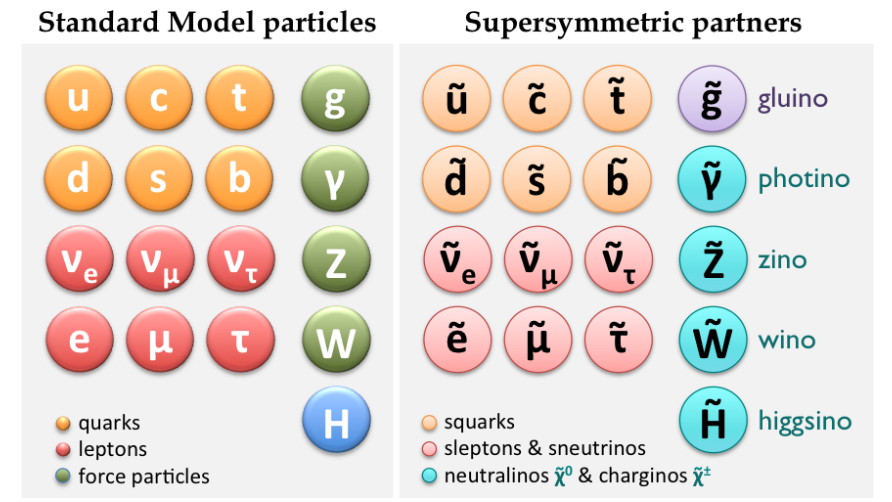
\includegraphics[width = 0.75\textwidth]{Figures/FromOnline/susy_particles.png}
    \caption{An illustration of the content of particles in the SM and sparticles in SUSY \cite{SUSYpic}.}
    \label{fig:smandsusy}
\end{figure}

In SUSY, we do not have to introduce any new gauge groups, which means we do not have to handle any new fundamental forces. Because of this we can, in a way, say that we can describe supersymmetry with the help of a supersymmetry operator $Q$ that alters the spin of the SM particles by $1/2$ and commutes with the gauge transformations of the SM: 
\begin{equation}
    \label{eq:SUSY}
    Q\ket{\mathrm{fermion}} = \ket{\mathrm{bosons}} \text{,   }  Q\ket{\mathrm{bosons}} =\ket{\mathrm{fermions}}.
\end{equation}

SUSY possibly provides a solution to the SM's hierarchy problem, which involves the need to reconcile the very different scales of electroweak symmetry breaking and the gravitational Planck scale ($M_{Pl}$). SUSY allows the unification of the electroweak and strong interactions, proposes dark matter particle candidates, and requires five Higgs bosons (three neutral and two charged ones). One of these proposed DM particles is the lightest supersymmetric particle (LSP) and is assumed to be stable. To make the LSP stable, we have constructed a new quantum number called R-parity such that no SUSY particles can decay into only SM particles. R-parity is defined as 

\begin{equation}
    \label{eq:Rparity1}
    P_{\mathrm {R} }=(-1)^{3B+L+2s}
\end{equation}

or

\begin{equation}
    \label{eq:Rparity2}
    P_{\mathrm {R} }=(-1)^{3(B-L)+2s},
\end{equation}

where $B$ is the baryon number\footnote{Baryon number is a conserved quantity in the SM and is defined by $\frac{1}{3}(n_q - n_{\Bar{q}})$, where $n_q$ is the number of quarks and $n_{\Bar{q}}$.}, $L$ is the lepton number\footnote{The lepton number tells us the difference between the number of leptons and anti-leptons. This is also conserved in the SM.} and $s$ is the spin of the particle. 

In addition to the LSP, we are going to look at some different SUSY particles in our processes, namely neutralino and chargino. They are a mixture of the sparticle components photino, zino, and neutral higgsino, and wino and the charged higgsino, respectively.


\begin{comment}

We know that the sparticles differ from the particles by $1/2$ spin, but that is almost the only difference when 

Supersymmetry allows for a connection between fermions and bosons by introducing a new set of particles. Each SM-particle has a sparticle, equal in all quantum numbers except a half unit difference in spin, i.e. the SM-fermions get a bosonic superpartner (denoted by an "s" in front of the name, e.g. electron $\rightarrow $ selectron) while the SM-bosons get a fermionic superpartner (denoted by "-ino" added to the end of the name, e.g. $W \rightarrow$ wino). All sparticles are denoted by a tilde above their symbol, e.g. selctron ($\tilde{e}$). If SUSY is a valid extension of the Standard Model, we know that it must be a broken symmetry where the particles and sparticles must have different masses although all the quantum numbers are equal. The sparticles must be heavier than their partner, or else we would already have been able to detect them in particle detectors, such as the ATLAS experiment. 

Supersymmetry offers a solution to the hierarchy problem, and when imposed as a local symmetry, gravity. According to Einsteins mass-energy equivalence equation ($E = mc^2$), we should be able to produce any particle in the universe as long as we collide them with a high enough amount of energy.





:
Production of pairs of sleptons, hypothetical supersymmetric partners of leptons, in the process pp→~l+~l-→ l+l-+χχ, where the DM candidate χ is the lightest neutralino (a mixture of photino, zino and higgsino), leading to a pair of leptons (e⁺e⁻ or µ⁺µ⁻) and missing transverse energy (MET).







The process I am looking at in this project is direct slepton production as shown in the Feynman diagram in figure \ref{fig:slepslep}. Production of pairs of sleptons, hypothetical supersymmetric partners of leptons, in the process $pp\rightarrow \tilde{l}^+\tilde{l}^- \rightarrow l^+l^-+ \chi \chi$, where the DM candidate $\chi$ is the lightest neutralino (a mixture of photino, zino and higgsino), leading to a pair of leptons ($e^+ e^-$ or $\mu^+ \mu^-$) and missing transverse energy (MET).



The same final state (l+l-+MET) above may be due to the production of a pair of lightest charginos χ±1 , a mixture of the wino (W-superpartner) and the charged higgsino (charged Higgs superpartner), through the process pp→ χ+1χ-1, followed by (i) slepton-mediated ( ~l+~l-/~ν~ν → l+l-  + ννbar + χχ) or (ii) W-mediated (W+W-→l+l-  + ννbar +χχ) decays into leptons and MET.



\textbf{To do:}
\begin{itemize}
    \item Fixing the hierarchy problem
    \item Superpartners
    \item Legg
\end{itemize}
\end{comment}



